\section{Related Work}
This section aims to present the theoretical background and related work relevant to this project.

\subsection{Domain Generalization}

Domain Generalization is a machine learning approach to enable machine learning models to generalize to new, unseen domains, without  access to the target domain data during the models training. Hereby Domain Generalization tries to learn generalized features from the source domain that can peform well even on unseen domains. This is particulary important for computer vision tasks - especially real world computer vision tasks, where the target domain data is subject to constant changes or is not even available at all, making it impossible to adapt a model continuously. \cite{liDeeperBroaderArtier2017,liuDEJAVUContinual2023,blanchardGeneralizingSeveralRelated2011}


Furthermore, Domain Generalization can be broken down into two: Multi-Source Domain Generalization and Single-Source Domain Generalization.
Multi-Source DG assumes that there is more than one relevant domain available, with the goal to use data from multiple sources to learn representations that are independent of different marginal distributions. \cite{blanchardGeneralizingSeveralRelated2011}
Single-Source DG, on the other hand, assumes that there is only one relevant domain available during training, 

The need to generalize well to new domains arises from the problem of domain shift. Domain shift can significantly worsen the performance of a model - especially DNNs - across different domains \cite{muandetDomainGeneralizationInvariant2013}. These shifts can be cause by a variety of factors. Common sources include:
\begin{itemize}
    \item \textbf{Image Style}: Is a major source of domain shifts, such as changes in colours, textures, lighting, etc \cite{zhouMixStyleNeuralNetworks2023}.
    \item \textbf{Environmental Conditions}: Changes in the environment, such as weather, time of day, or camera settings, can also cause domain shifts \cite{schwonbergAugmentationbasedDomainGeneralization2023}.
    \item \textbf{Visual Abstraction}: Datasets can vary in their level of abstraction, from relaistic photos over to abstracts sketches or paintings \cite{liDeeperBroaderArtier2017}.
\end{itemize}



Hereby Domain Generalization needs to be distinguished from Domain Adaptation, as both paradigms address the challenge of domain shifht. While Domain Adaptation aims to adapt a model to perform well on a specific target domain, by reducing the performance gapbetween the source and target domains. Domain Generalization aims to learn domain-invariant features such that the model can perform well on new unseen target domains, without the need to see the target domain data during training \cite{liDeeperBroaderArtier2017}. Conversly, Domain Adaptation methods typically assume the access to the target domain data during training and trying to adapt the model from the source domain to perform well on the target domain \cite{liuDEJAVUContinual2023, wangDeepVisualDomain2018}. 

To quantify the performance of a model benchmarks and evaluation protocols have been developed. Common benchmarks include:
\begin{itemize}
    \item \textbf{PACS}: \cite{liDeeperBroaderArtier2017} This is commonly used benchmark including four domains: photo, art painting, cartoon and sketch. It contains 9991 images across seven categories. The domains are designed to be maximally disctinct, covering a wide range of visual styles - from realistic photos to abstract sketches.
    \item \textbf{Office-Home}: \cite{venkateswaraDeepHashingNetwork2017} This dataset also contains four domains: art, clipart, product and real-world. With 15,500 images across 65 categories it is larger than PACS. The contents are related to objects found in office and home environments.
    \item \textbf{VLCS}: Consits out of four domains: PASCAL VOC2007 (V), LabelMe (L), Caltech-101 (C), and SUN09 (S). It contains 10729 images across five classes. %cite FangUnbiasedMetricLearning2013

\end{itemize}
Common evaluation protocols include:
\begin{itemize}
    \item \textbf{Leave-One-Domain-Out (LODO)}: Is a common evaluation protocol where one domain is held out as the target domain and the model is evaluated on the remaining domains. \cite{liDeeperBroaderArtier2017}
    \item \textbf{Direct Transfer}: Is another approach where the model is trained on one dataset (e.g. MSMT17) and then evaluated on another dataset (e.g. Market1501), without any finetuning on the target domain. \cite{chongLearningDomainInvariant2021}
\end{itemize}

Note all of the above mentioned datasets are also part of the \textbf{DomainBed} benchmark suite created by \cite{gulrajaniSearchLostDomain2020} for Domain Generalization, which includes more datasets, evaluations protocol and algorithms for Domain Generalization.

The most common approaches to Domain Generalization according to a survery conducted by \cite{zhouDomainGeneralizationSurvey2022} are:
\begin{itemize}
 \item \textbf{Domain Alignment}: Most current domain generalization methods fall into the domain alignment category, aiming to reduce disparities between source domains to learn representations that are invariant across them
 \item \textbf{Meta-Leraning}: This approach, also known as 'learning to learn', trains a model on a variety of learning tasks to enable it to solve new learning tasks more effectively. In the context of DG, it helps the model generalize to new domains by learning from domain shifts in the source data.
 \item \textbf{Data Augmentation}: Involves expanding the original dataset with new transformed data, simulating domain shifts.
\end{itemize}

In the latter category two techniques also employed in this project are situtated:
Image Transformation and Feature-Based Augmentation.

Image Transformations are a common technique for data augmentation, where the original image is transformed by methods such as rotation, scaling, cropping, color jittering, etc.
On the other hand, Feature-Based Augmentation rely on mixing the CNN feature statistics across different domains - precisely the appraoch in the focus of this project MixStyle (\cite{zhouMixStyleNeuralNetworks2023}), while others approaches may also combine domains in both feature as well as pixel space.

Now let's dive deeper into the Feature Space.
\subsection{The Role of the Feature Space}
The feature space in CNNs refers to the multidimensional representation of the the data that the network learns durinc training. This is crucial for the classification tasks performed by CNNs, as it isolates the features extracted from input images, allwoing the model to differentiate between various categories, whether it be domains or classes.
Hereby, CNNs automatically extract features from images through their convolutional layers, creating a hierachical representation. With each layer capturing different levels of abstraction - starting from low-level features such as edges and textures, then moving to more complex features like shapes and eventually to semantic representations like structures or even obejects in deeper layers. \cite{zeilerVisualizingUnderstandingConvolutional2013,goodfellowDeepLearning2016}

\begin{figure}[ht]
    \centering
    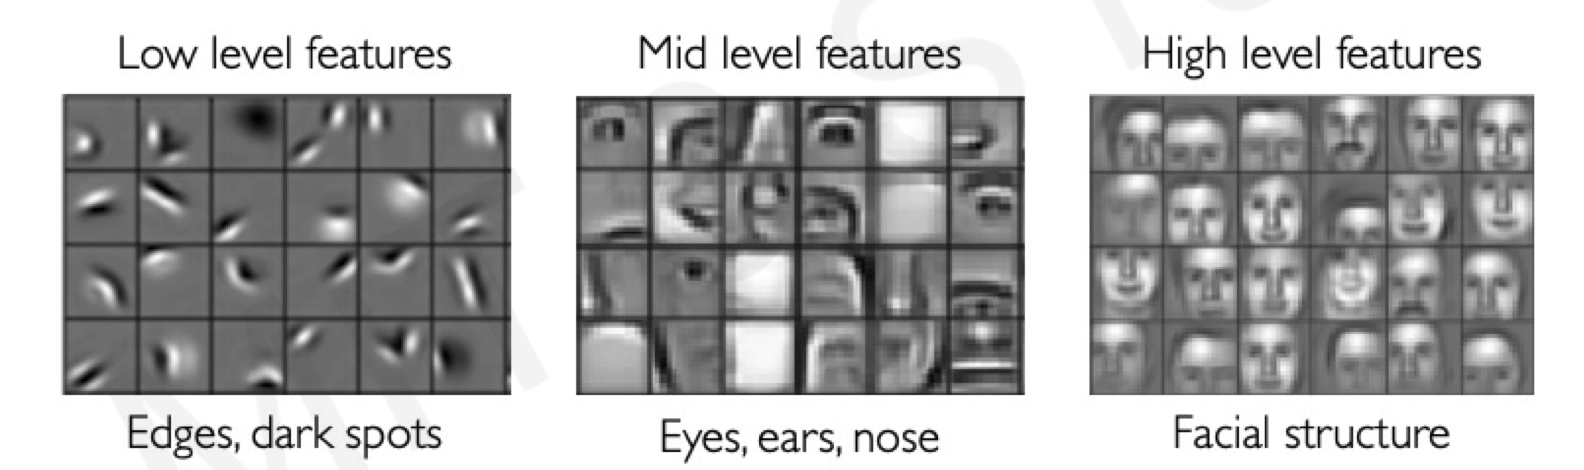
\includegraphics[width=0.85\textwidth]{images/Learning-Feature-Representation.png}
    \caption{Illustration of feature abstraction hierarchy in CNNs, from low-level (edges) to high-level (semantic object parts). Adapted from \cite{alexanderaminiMITIntroductionDeep2025}.}
    \label{fig:Hierachy_of_Features}
\end{figure}
This hierachy show why shallow layers are often more domain-specific, as they are prone to capturing texture or lighting, while deeper layer are more semantic and thus domain-invariant. Feature-space domain generalization methods like MixStyle \cite{zhouMixStyleNeuralNetworks2023} start their approach there.
Fature representations derived from CNNs, ofter form domain-specific clusters in the latent space. This in particular is problematic for Domain Generalization, where the models needs to learn representations that are invariant to such domain cues. \cite{zhouDomainGeneralizationSurvey2022}

\begin{figure}[!htb]
    \centering
    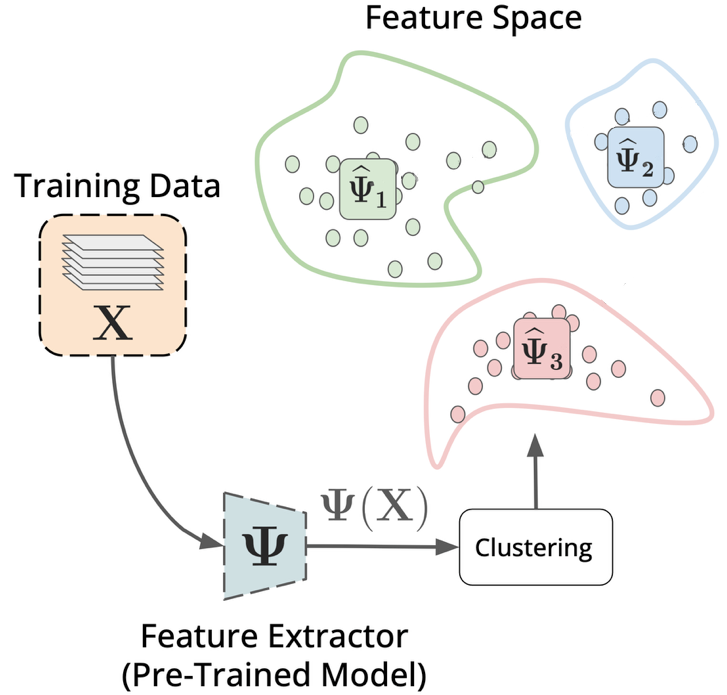
\includegraphics[height=0.25\textheight]{images/Pipeline-Feature_Space.png}
    \caption{A model pipeline showing input images from different domains processed by a pretrained feature extractor, producing clustered representations in feature space. Image from \cite{thomasWhatsLatentLeveraging2025}, modified.}
    \label{fig:Pipeline_Feature_Space}
\end{figure}
Clustered representations usually refelct the charecteristics of the source domain. Without any intervention, models trained on these clustered representations might sturggle to generalize to new domains.
One effective way to address this issue is by utilising transfer learning, by reusing pretrained models.
\subsection{Transfer Learning}
Transfer learning refers to the process of leveraging knowledge obtained from one task or domain to improve performance on a different, yet related, task. In the context of computer vision, it often involves using models pretrained on large-scale datasets — such as ImageNet — and adapting them to new tasks with limited data.

This approach is particularly relevant to Domain Generalization, where the goal is to generalize to an unseen target domain without access to its data during training \cite{gulrajaniSearchLostDomain2020,liDeeperBroaderArtier2017}. Transfer learning can support this objective by providing models with general-purpose representations learned from diverse visual categories and conditions.

Convolutional Neural Networks (CNNs) pretrained on large datasets tend to capture a hierarchy of features as seen in figure \ref{fig:Hierachy_of_Features} — from low-level structures like edges and textures to high-level semantic patterns. These pretrained networks are often used as \textbf{feature extractors} enabling downstream models to build upon robust and transferable representations rather than learning from scratch. Furthermore, beyond improved sampling efficiency, transfer learning can also stabilize training and reduce overfitting, especially in cases where the available training data is limited or varies substantially across domains. Thus, transfer learning provides a useful foundation for addressing domain shift in Domain Generalization settings, even though it is not exclusive to them.

\subsection{Freezing}
Another concept that is independent of Domain Generalization, but may come useful in the context of Domain Generalization, is the concept of freezing.
Freezing refers to the practice of keeping certain layers of a neural network, in particular layers that contain batch normalization, fixed during the training process. This technique can be employed for Domain Generalization tasks, by preventing the batch normalization statistics from beeing update with data from diverse source domain, the model can btter reatain its robust, pre-trained features, which is crucial to achieve effective domain generalization. \cite{gulrajaniSearchLostDomain2020,zhouMixStyleNeuralNetworks2023}


\subsection*{Summary}
In summary, DG provides a more demanding but often more practical solution than DA for creating models that are robust to the diverse and unpredictable domain shifts encountered in real-world scenarios.

\clearpage